\documentclass{cmppgr}
\usepackage[utf8]{inputenc}
\usepackage{pdfpages}
\usepackage{listings}
\usepackage[margin=0.5in]{geometry}
\usepackage{caption}
\usepackage{datetime}

\definecolor{pblue}{rgb}{0.13,0.13,1}
\definecolor{pgreen}{rgb}{0,0.5,0}
\definecolor{pred}{rgb}{0.9,0,0}
\definecolor{pgrey}{rgb}{0.46,0.45,0.48}

\lstset{
  language=Java,
  numbers=left,
  showspaces=false,
  showtabs=false,
  breaklines=true,
  showstringspaces=false,
  breakatwhitespace=true,
  commentstyle=\color{pgreen},
  keywordstyle=\color{pblue},
  stringstyle=\color{pred},
  basicstyle=\ttfamily,
  breaklines=true,
  postbreak=\mbox{\textcolor{red}{$\hookrightarrow$}\space},
}
\title{An experimental assessment of decision trees and decision tree ensembles}
% change this to match your student number
\name{Student number: 100238596. Blackboard ID: pxh18ksu}
\begin{document}
\maketitle

\section {Introduction}

Start with the aims of the paper, a description of the hypotheses you are testing and an overview of the structure. Include in this your prior beliefs as to what you think the outcome of the test will be, with some rationalisation as to why. So, for example, do you think attribute evaluation will make a difference? Can you find any published literature that claims to answer any of the questions?

\section{Data Description}

An overview describing the data, including data characteristics summarised in a table (number of attributes, number of train/test cases, number of classes, class distribution). For your case study data set you should have more detail, including a description of the source of the data and the nature of the problem the data describes. Look for references for similar types of problem.


\section {Classifier Description}

Include a description of your C45Coursework classifier, including details of design choices you made and data structures you employed. You should include an example of how to use the classifier with the refinements you have included. Also provide an overview of the other classifiers you use in the case study, including references.

\section {Results} 

A description of the experimental procedure you used and details of the results. Remember, graphs are good. There should be a subsection for each hypothesis. The case study section should go into greater depth and remember, accuracy is not the only criteria.



   \begin{figure}[hb]
    	\centering
        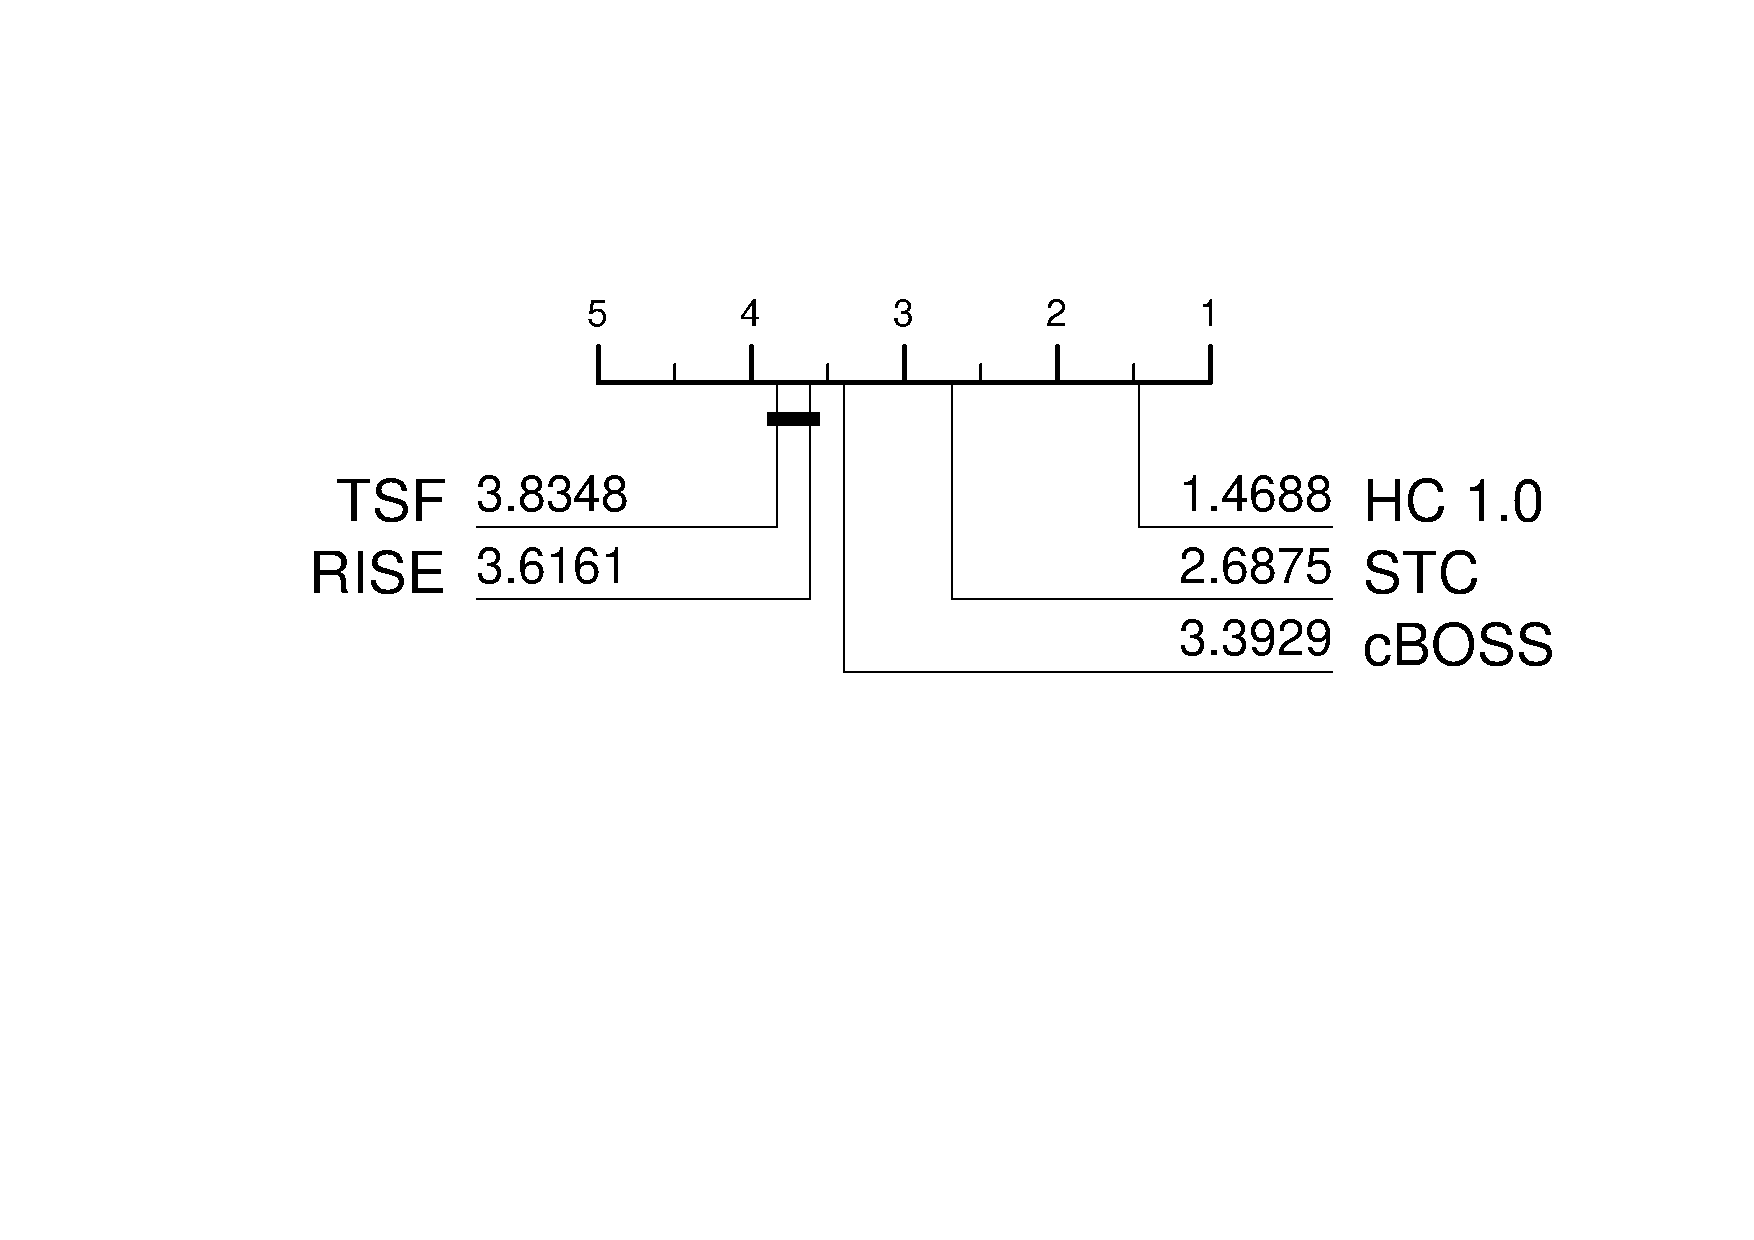
\includegraphics[width=\linewidth,trim={2cm 8cm 2cm 4cm},clip]{cd_HC-Analysis_ACCS.pdf}
        \caption{An example Critical difference diagram taken from~\cite{bagnall20hivecote1}}
        \label{fig:hc1.0}
    \end{figure}
    

\section{ Conclusions}

How do you answer the questions posed? Are there any biases in your experiment and if so, how would you improve/refine them?
%Describe your solution here
% for the paper, it is probably best to write it in its own overleaf project then import the pdf here

\bibliographystyle{plain}
\bibliography{example} 

\end{document}